\chapter{Results and Discussions}\label{ch:results}
This chapter is organized as follows: Section \ref{sec:ch4_desc_stat} will discuss the results of the descriptive statistics; Section \ref{sec:ch4_morphological_analysis} will discuss the results on the morphological analyses; Section \ref{sec:ch4_structural_analysis} will discuss the structural analyses including the Mathematical structures of the Qur'\=an; Section \ref{sec:ch4_topic_modeling_result} will discuss the results for thematic analyses using both statistical and Large Language models; and finally, 
Section \ref{sec:ch4_relating_islamic_texts} will discuss the use of other Islamic texts that will help in adding more contexts for the Large Language models.
\section{Descriptive Statistics}\label{sec:ch4_desc_stat}
This section will focus on the results of the descriptive statistics of the Qur'\=an's \arb[trans]{ayAt} \arb{ayAt} (verses) and \arb[trans]{kalimat} \arb{kalimAt} or words. Figure \ref{fig:ch4_ayah_word_count} visualizes the frequency of the \arb[trans]{ayAt} \arb{ayAt} and words of the Qur'\=an using a combinations of bar, density, and box plots. The figure is divided into three main parts. The first part is the statistics of the \arb[trans]{ayAt}'s \arb{ayAt} count. It can be seen that in terms of the number of verses, it is generally decreasing just like what the Muslims observed. Table \ref{tbl:desc_stats} summarizes the necessary statistics of Figure \ref{fig:ch4_ayah_word_count}. From the said table, there are 39 \arb[trans]{ayAt} \arb{ayAt} to expect based on the median statistics, and there are about 55 \arb[trans]{ayAt} \arb{ayAt} to expect per \textit{s\=urah} \arb{sUraT} based on the mean statistics. The reason the mean is higher than the median follows from the fact that there are surahs that can be considered outlier because of the large number of \arb[trans]{ayAt} \arb{ayAt}. The annotation on the \textit{s\=urah} \arb{sUraT} with the highest number of \arb[trans]{ayAt} \arb{ayAt} are indicated in Figure \ref{fig:ch4_ayah_word_count}. These \textit{s\=urah} \arb{sUraT} pushes the mean to higher number than the median. Indeed, these \textit{s\=urahs} \arb{sUr} have stretched the shape of the density and the box plots to higher values, suggesting that the data points are more varied. The width of the density and the box plots is measured by the variance and the standard deviation, which is simply the square root of the variance. 

\begin{table}
    \caption{Descriptive statistics of the \arb[trans]{ayAt} \arb{ayAt} counts and the counts of its words}
    \label{tbl:desc_stats}
    \begin{tabularx}{\textwidth}[!h]{XXXX}
        \toprule
        Count Data&Mean&Median&Std. Deviation\\
        \midrule
        Ayahs&54.70&39&53.21\\
        Words&679.20&344&931.18\\
        Words per Ayah&10.27&8.23&6.35\\
        \bottomrule
    \end{tabularx}
\end{table}


\begin{figure}[!t]
    \centering
    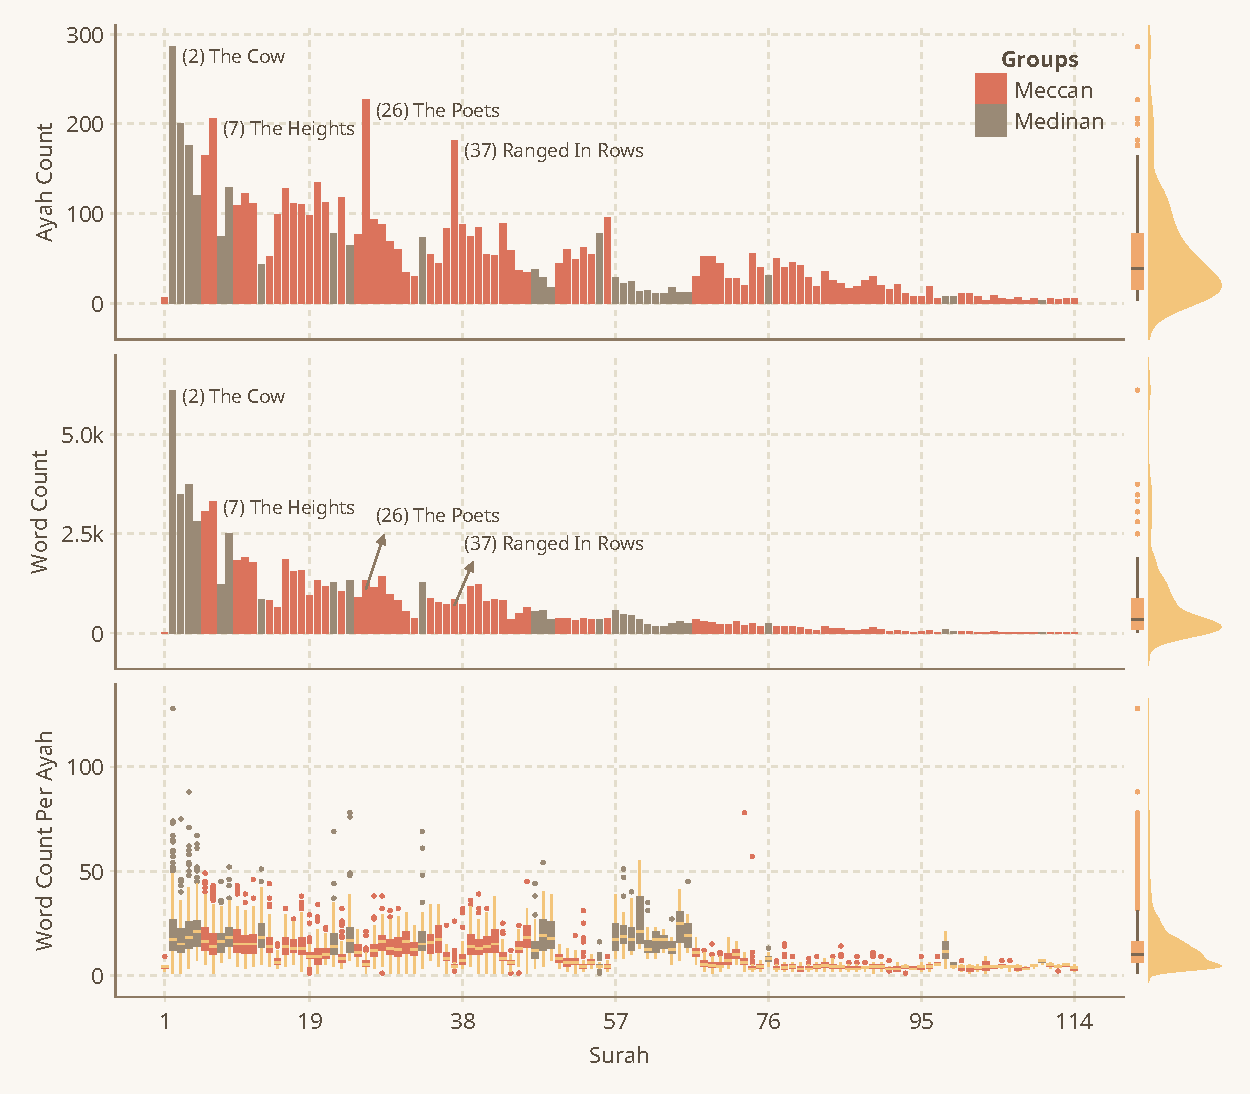
\includegraphics[width=\textwidth]{img/plot1.pdf}
    \caption{Statistics of the words and \arb[trans]{ayAt} \arb{ayAt} (verses) of the Qur'\=an}
    \label{fig:ch4_ayah_word_count}
\end{figure}

\begin{figure}[!t]
    \centering
    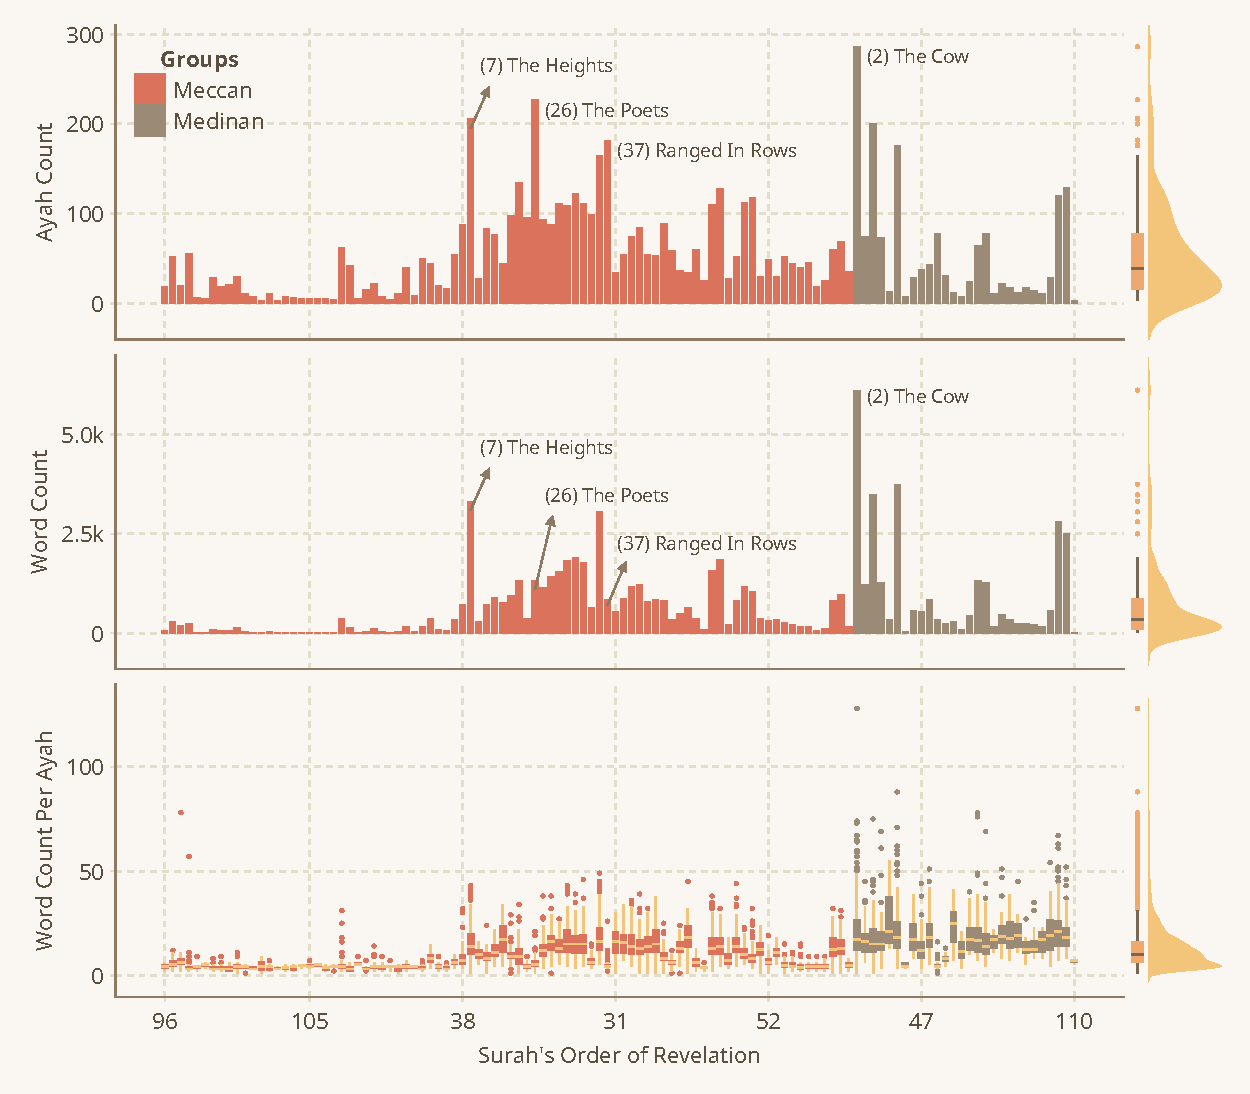
\includegraphics[width=\textwidth]{img/plot2.pdf}
    \caption{Statistics of the words and \arb[trans]{ayAt} \arb{ayAt} (verses) of the Qur'\=an according to revelation order}
    \label{fig:ch4_ayah_word_count_rev_order}
\end{figure}

\subsection{Verses}\label{sec:ch4_desc_stat_verse}
\section{Morphological Analysis}\label{sec:ch4_morphological_analysis}
\section{Structural Analysis}\label{sec:ch4_structural_analysis}
\subsection{Concentric Structure}
\subsection{Discussions on Islamic Philosophy of Qur'\=an's Structural Analysis}
\newpage
\section{Topic Modeling}\label{sec:ch4_topic_modeling_result}
\subsection{Latent Dirichlet Allocation}
\subsection{Bidirectional Encoder Representation from Transformer}
\subsection{Generative Pre-Trained Transformer}
\section{Relating to other Islamic Texts and Analyses}\label{sec:ch4_relating_islamic_texts}
\subsection{Retrieval-Augmented Generation Approach}
\section{Limitations of the Models}